\section{BackEnd}
\subsection{Introduzione}
Questa parte del prodotto è orientata all'uso da parte di tutto il software che dipenda dalle REST API di BlockCovid. Nel sistema implementato da DPCM2077, dipendono dalle REST API l'applicazione mobile per gli utenti e la web-app per gli amministratori.

\subsubsection{Scopo}
Il backend permette in BlockCovid, all'app utenti e alla web-app, di fornire ad utenti e amministratori gli strumenti necessari per il funzionamento. Essendo il backend sviluppato in maniera separata ed indipendente dall'applicazione mobile e la web-app, la modalità in cui è implementato non è rilevante per gli sviluppatori \textit{bc19-android} e \textit{bc19-webapp}.
\\
\\
Le funzionalità offerte dal backend sono quelle indicate nella sezione \textbf{§7 REST API} del Manuale. Per avere ulteriori informazioni si invita quindi a visitare la sezione indicata.


\subsection{Requisiti e installazione}
Per poter sviluppare ed aggiungere funzionalità al backend del sistema BlockCovid, sono necessari gli strumenti indicati in questa sezione.

\subsubsection{Prerequisiti hardware e software}
È consigliato l'utilizzo di un server con risorse sufficienti per il funzionamento del backend. Questo dipende molto dalla mole di utenti e, per non incorrere in problemi in fase di sviluppo, è consigliato avere risorse hardware equivalenti ad un processore quad-core e 8 GB di RAM.
\\\\
Il sistema operativo di riferimento per lo sviluppo è Ubuntu 18.04 LTS e Ubuntu 20.04 LTS.

\subsubsection{Ottenimento codice sorgente}
Per scaricare il codice sorgente è necessario \textbf{Git}. Se non si dispone di Git è possibile scaricarlo seguendo quanto indicato nella sezione \textbf{§4.2.4}. Per scaricare il progetto, invocare il seguente comando da terminale: \textit{git clone https://github.com/DPCMGroup/bc19-api.git}.

\subsubsection{Linguaggi utilizzati}
\paragraph{Python}
Il backend è stato sviluppato utilizzando il linguaggio di programmazione python, in particolare è stata utilizzata la versione python 3.6 per lo sviluppo del progetto.

\subparagraph{Installazione di python}
Per l'installazione di python è sufficiente scaricare ed installare il pacchetto, rispettivo al proprio sistema operativo, dal \href{https://www.python.org/downloads/}{sito ufficiale}.

\subparagraph{Installazione dependency}
Il backend è strutturato secondo quanto messo a disposizione dal framework Django e inoltre utilizza molte altre librerie. I pacchetti utilizzati sono definiti nel file \textbf{requirements.txt} e sono necessari per il corretto funzionamento del servizio.\\
Per installare i pacchetti è necessario posizionarsi con il terminale allo stesso livello del file requirements.txt. Successivamente è sufficiente eseguire il seguente comando: \textit{pip install -r requirements.txt}

\paragraph{YAML}
Il backend usufruisce dei workflow messi a disposizione da GitHub, chiamati GitHub Actions. Il workflow è definito in un file yml, in cui sono specificate le azioni da eseguire per compilare o eseguire gli unit test.
\\YAML viene utilizzato anche per la definizione del docker-compose su cui verrà eseguito Django.

\subsubsection{Source Code Management}
Per poter effettuare il versionamento del codice sorgente è richiesto l'utilizzo di \textbf{Git}. Se non si dispone di Git è possibile scaricarlo ed installarlo seguendo le istruzioni del \href{https://git-scm.com/downloads}{sito ufficiale}.

\subsubsection{Database}
Il backend per il suo corretto funzionamento ha bisogno di interfacciarsi ad un database. Per la sua configurazione fare riferimento alla sezione \textbf{§5}.
Nel caso in cui si volesse cambiare il database a cui Django si interfaccia, è necessario cambiare le impostazioni del file \textit{settings.py} nella sezione \textit{DATABASE}. È consigliato seguire le istruzioni del \href{https://docs.djangoproject.com/en/3.2/ref/databases/}{sito ufficiale} di Django.
\\
\\
Django è configurato per l'utilizzo di un database MariaDb e necessita del file my.cnf dove all'interno sono definite le credenziali e l'endpoint di accesso. Il file deve essere allo stesso livello di \textit{manage.py}.

\subsubsection{Docker container}
Docker viene utilizzato per l'esecuzione del servizio in produzione.
\paragraph{Installazione di Docker su Windows}
È possibile installare Docker su Windows visitando il suo sito ufficiale, alla \href{https://hub.docker.com/editions/community/docker-ce-desktop-windows}{seguente pagina}. La guida all'installazione e al primo utilizzo è presente nello stesso link in cui si scarica l'eseguibile per l'installazione.
\paragraph{Installazione di Docker su MacOS}
L'installazione per MacOS è identica a quella per Windows, ma la pagina a cui scaricarlo si trova a \href{https://hub.docker.com/editions/community/docker-ce-desktop-mac}{questo link}.
\paragraph{Installazione Docker Linux}
È possibile installare Docker su Ubuntu seguendo le guide presenti sul sito ufficiale, disponibili a \href{https://docs.docker.com/engine/install/ubuntu/}{questo indirizzo}.

\subsubsection{Esecuzione}
Attualmente sono presenti due modi per eseguire il backend:
\begin{itemize}
	\item Tramite linea di comando;
	\item Tramite l'utilizzo di docker (consigliato).
\end{itemize}
\paragraph{Linea di comando}
Per eseguire il backend tramite linea di comando, è necessario posizionarsi allo stesso livello del file \textit{manage.py} ed eseguire il comando \textit{python manage.py runserver 8000}.\\Questo rende disponibile il servizio sulla porta 8000 dell'host.
\paragraph{Docker}
Per eseguire il backend tramite docker, è necessario posizionarsi allo stesso livello del file \textit{docker-compose.yml} ed eseguire il comando \textit{docker-compose up}. Docker si occuperà di scaricare tutti i pacchetti necessari per l'esecuzione e renderà disponibile il servizio sulla porta 8000 dell'host.
\subsection{Architettura}
Nel backend è stato utilizzato il design pattern che utilizza Django, che si ispira al Model-View-Controller (MVC), e si chiama Model-Template-View.
In questo caso il \textit{Model} rispecchia la gerarchia dei dati presenti nel database, la \textit{View} si occupa della elaborazione di questi dati e il \textit{Template} è, appunto, il template utilizzato come risposta.
\begin{figure}[H]
	\centering
	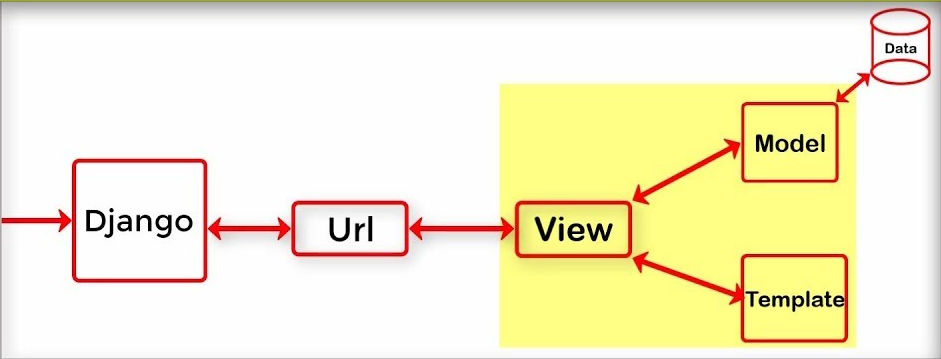
\includegraphics[width=16cm]{res/images/mvt.png}
	\caption{Model-Template-View}
	\label{fig:Model-Template-View}
\end{figure}